\documentclass[10pt,xcolor=pst,aspectratio=169]{beamer}

\usepackage{etex}

%\usetheme{Boadilla}
%\usecolortheme{wolverine}
\usecolortheme{dolphin}
%\setbeamercovered{transparent}
%\setbeamercolor{block body}{bg=yellow}

\addtobeamertemplate{navigation symbols}{}{%
\usebeamerfont{footline}%
\usebeamercolor[fg]{footline}%
\hspace{1em}%
\insertframenumber/\inserttotalframenumber
}

\usepackage[utf8]{inputenc}
\usepackage[english,russian]{babel}
\usepackage[OT1]{fontenc}
\usepackage{amsmath}
\usepackage{amsfonts}
\usepackage{amssymb}
\usepackage{graphicx}
\usepackage{wrapfig}
\usepackage[3D]{movie15}
\usepackage{animate}
\usepackage{ragged2e}
\usepackage{listings}
\usepackage{color}
\usepackage{pst-all}

\usepackage{tikz,pgfplots}
\usetikzlibrary{
	mindmap,
	arrows, % стрелки
	shapes.misc, % фигуры
	chains, % цепочки
	positioning, % позиционирование элементов
	scopes, % создание дополнительных веток
	shadows % тени
	}

\graphicspath{{pic/}}

\author{\textbf{Губкин А.С.}}

\title[Численные методы в физике]{Численные методы в физике}

\logo{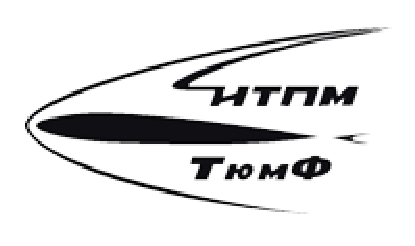
\includegraphics[width=0.1\linewidth]{LOGO_2.EPS}}

\institute[ТюмФ ИТПМ СО РАН]{Тюменский филиал Института теоретической и прикладной механики\\ им. С. А. Христиановича СО РАН, г. Тюмень}

%\date{6 октября 2015 г.}

\begin{document}

\lstset{ %
	language=[ANSI]C++,                 % выбор языка для подсветки (здесь это С++)
	keywordstyle=\color{blue},
	commentstyle=\color{gray},
	basicstyle=\scriptsize,
%basicstyle=\small\sffamily, % размер и начертание шрифта для подсветки кода
	numbers=left,               % где поставить нумерацию строк (слева\справа)
	numberstyle=\tiny,           % размер шрифта для номеров строк
%stepnumber=1,                   % размер шага между двумя номерами строк
	numbersep=4pt,                % как далеко отстоят номера строк от подсвечиваемого кода
%backgroundcolor=\color{white}, % цвет фона подсветки - используем \usepackage{color}
	showspaces=false,            % показывать или нет пробелы специальными отступами
	showstringspaces=false,      % показывать или нет пробелы в строках
	showtabs=false,             % показывать или нет табуляцию в строках
	frame=single,              % рисовать рамку вокруг кода
%tabsize=2,                 % размер табуляции по умолчанию равен 2 пробелам
	captionpos=t,              % позиция заголовка вверху [t] или внизу [b] 
	breaklines=true,           % автоматически переносить строки (да\нет)
	breakatwhitespace=true, % переносить строки только если есть пробел
	escapeinside={\%*}{*)}   % если нужно добавить комментарии в коде
}

%SLIDE #
\begin{frame}

	\transdissolve[duration=0.1]
	\titlepage

\end{frame}

%SLIDE #
\begin{frame}{Линейные волны, распространяющиеся без затухания}

	\transdissolve[duration=0.1]
	\justifying
	\large

    Рассмотрим далее общие свойства линейных волн, распространяющихся в одномерном пространстве без диссипации. В этом случае независимыми переменными являются $t$ и $x$. Волновая система может описываться одной или более зависимыми переменными; рассмотрим пока одну переменную и обозначим ее $u$.\\

    (Иногда употребялют оборот волны с диссипацией и дисперсией -- с точки зрения физики это не верно)

\end{frame}

%SLIDE #
\begin{frame}{Фаза и фазовая скорость}

	\transdissolve[duration=0.1]
	\justifying
	\large

    Рассмотрим волновое изменение зависимой переменной $u \left( x, t \right)$ в виде:

    \[
		u \left( x, t \right) = u_{0} \operatorname{Re} \left\lbrace e^{i \theta} \right\rbrace = u_{0} \cos \left( \theta \right) .
	\]

    $\theta$ -- фаза, линейная по независимым переменным

    \[
        \theta = k x - \omega t + \alpha,
    \]

    $k$ -- волновое число, $\omega$ -- круговая частота.

    Фаза будет оставаться постоянной для наблюдателя, который движется со скоростью

    \[
        \frac{d x}{d t} = \frac{\omega}{k} = c.
    \]

    Действительно

    \[
        \frac{d \theta}{d t} = \frac{\partial \theta}{\partial t} + \frac{d x}{d t} \frac{\partial \theta}{\partial x} = - \omega + \frac{\omega}{k} k = 0.
    \]

\end{frame}

%SLIDE #
\begin{frame}{Дисперсионное соотношение}

	\transdissolve[duration=0.1]
	\justifying
	\large

    В общем случае для распространяющихся волн существует функциональное соотношение $f \left( \omega, k \right)$, связывающее частоту и волновое число. Обычно это соотношение имеет вид зависимости частоты от волнового числа $k$:

    \[
        \omega = W \left( k \right).
    \]

    Соотношение такого типа обычно называют дисперсионным соотношением или уравнением.

    Тогда \textbf{фазовая скорость} также зависит от волнового числа:

    \[
        c = \frac{\omega}{k} = \frac{W \left( k \right)}{k}.
    \]

    В случае, когда фазовая скорость не зависит от волнового числа (или от частоты), говорят, что волна распространяется без дисперсии. В таком случае функция $W$ имеет простой вид:

    \[
        W \left( k \right) = c k.
    \]

\end{frame}

%SLIDE #
\begin{frame}{Интеграл Фурье}

	\transdissolve[duration=0.1]
	\justifying
	\large

	Пусть задано начальное распределение $u \left( x, 0 \right)$. Если это начальное распределение не гармонично, то его можно представить с помощью интеграла Фурье как суперпозицию синусоидальных функций.

    \[
        u \left( x, 0 \right) = \frac{1}{2 \pi} \int\limits_{-\infty}^{\infty} \bar{u} \left( p, 0 \right) e^{i p x} dp ,
    \]

    \[
        \bar{u} \left( p, 0 \right) = \int\limits_{-\infty}^{\infty} \bar{u} \left( x, 0 \right) e^{- i p x} dx .
    \]

\end{frame}

%SLIDE #
\begin{frame}{Дисперсия}

	\transdissolve[duration=0.1]
	\justifying
	\large

    Поскольку система предполагается линейной, каждая из гармонических компонент изменяется как $e^{i \theta}$ c частотой $W \left( k \right) = c k$. Полное решение в любой последующий момент времени $t$ может быть получено путем обратного преобразования Фурье.\\

    В бездисперсионном случае этот процесс вновь приводит к начальному распределению, смещенному на расстояние $c t$. То есть, решение можно выразить в виде

    \[
        u \left( x, t \right) = u \left( x - c t, 0 \right).
    \]

Если же волна распространяется с дисперсией, то рассуждения теряют силу. В этом случае каждая компонента Фурье распространяется со своей скоростью.

\end{frame}

%SLIDE #
\begin{frame}{Групповая скорость}

	\transdissolve[duration=0.1]
	\justifying
	\large

    Производная от правой части дисперсионного соотношения имеет размерность скорости

    \[
        C \left( k \right) = \frac{d W}{d k}.
    \]

    Это величина называется \textbf{групповой скорость}.

\end{frame}

%SLIDE #
\begin{frame}{Интерпретация групповой скорости}

	\transdissolve[duration=0.1]
	\justifying
	\large

    Выберем некоторое значение $k$ и соответствующее ему значение $\omega = W \left( k \right)$ как исходные величины и допустим, что кволновому числу добавляется малое возмущение $\pm \triangle k$. Соответствующее возмущенное значение частоты может быть аппроксимировано первыми двумя членами ряда Тейлора:

    \[
        \omega + \triangle \omega = W \left( k + \triangle k \right) \approx \omega + C \triangle k .
    \]

    \[
        \omega - \triangle \omega = W \left( k - \triangle k \right) \approx \omega - C \triangle k .
    \]

    Соответствующие фазы

    \[
        \theta_{+} = \left( k + \triangle k \right) x - \left( \omega + \triangle \omega \right) t = \theta + \triangle k \left( x - C t \right) .
    \]

    \[
        \theta_{-} = \left( k - \triangle k \right) x - \left( \omega - \triangle \omega \right) t = \theta - \triangle k \left( x - C t \right) .
    \]

\end{frame}

\begin{frame}{Интерпретация групповой скорости}

	\transdissolve[duration=0.1]
	\justifying
	\large

    Решение, соответствующее этим двум фазам

    \[
        \begin{split}
            u \left( x, t \right) & = u_{+} \left( x, t \right) + u_{-} \left( x, t \right) = u_{0} \left( \cos \left( \theta_{+} \right) + \cos \left( \theta_{-} \right) \right) = \\
            & = u_{0} \left( \cos \left( \theta + \triangle k \left( x - C t \right) \right) + \cos \left( \theta - \triangle k \left( x - C t \right) \right) \right) = \\
            & = 2 u_{0} \cos \left( \theta \right) \cos \left( \triangle k \left( x - C t \right) \right) .
        \end{split}
    \]

    Его можно рассматривать как волну с исходными волновым числом и частотой, модулированную по амплитуде множителем $\cos \left( \triangle k \left( x - C t \right) \right)$.

    \begin{center}
        \begin{tikzpicture}
        \begin{axis}[
	        title=Solution,
	        xlabel={$x$},
	        ylabel={$u \left( x, t \right)$},
	        minor tick num=0,
	        height=0.4\paperheight, 
	        width=0.6\paperwidth,
	        xmin=0,
	        xmax=3*pi,
	        ymin=-1.1,
	        ymax=1.1
        ]
        \addplot[
            blue,
            very thick,
            domain=0:3*pi,
            samples=100
        ] {cos(deg(x))};
        \addplot[
            red,
            very thick,
            domain=0:3*pi,
            samples=100
        ] {-cos(deg(x))};
        \addplot[
            black,
            very thick,
            domain=0:3*pi,
            samples=1000
        ] {cos(deg(x))*cos(deg(20*x))};
        \end{axis}
        \end{tikzpicture}
    \end{center}

\end{frame}

\begin{frame}{Интерпретация групповой скорости}

	\transdissolve[duration=0.1]
	\justifying
	\large

    

\end{frame}

%SLIDE #
\begin{frame}{Диссипация и дисперсия численного решения}

	\transdissolve[duration=0.1]
	\justifying
	\large

	Определим диссипацию и диспесиию для дифференциального волнового уравнения. Возьмем решение в виде:

	\[
		u(x, t) = u_{0} \exp{(i (\omega t - k x))},
	\]

	где $\omega = 2 \pi \nu$ -- круговая частота, $k = 2 \pi / \lambda$ -- волновое число.\\

	Подставив это решение в волновое уравнение, получим зависимость $\omega = \omega(k)$, которая называется \textbf{дисперсионным соотношением}.\\

	Если $\omega$ -- комплексное число, волна затухает!

	\[
		\exp{((- Im \omega) t)} = \exp{(- \gamma t)}.
	\]

\end{frame}

%SLIDE #
\begin{frame}{Фазовая и групповая скорость}

	\transdissolve[duration=0.1]
	\justifying
	\large

	\textbf{Фазовая скорость} -- это скорость, с которой движется фаза или отдельной гармоники:

	\[
		\frac{Re \omega}{k} = c_{f}.
	\]

	\textbf{Групповая скорость} -- это скорость волнового пакета, состоящего из гармонических волн с близкими волновыми числами (Передача энергии осуществляется с групповой скоростью!):

	\[
		\frac{d}{d k} Re \omega = c_{g}.
	\]

\end{frame}

%SLIDE #
\begin{frame}{Дисперсия волн}

	\transdissolve[duration=0.1]
	\justifying
	\large

	Если фазовая/групповая скорость зависит от $k$, то гармоники с разными волновыми числами распространяются с разными скоростями. Такое явление называется \textbf{дисперсией}.

\end{frame}

%SLIDE #
\begin{frame}{Пример №1}

	\transdissolve[duration=0.1]
	\justifying
	\large

	\[
		\frac{\partial^{2} u}{\partial t^{2}} = c^{2} \frac{\partial^{2} u}{\partial x^{2}} \Rightarrow - \omega^{2} = - c^{2} k^{2} \Rightarrow \omega = c k \Rightarrow \frac{Re \omega}{k} = \frac{d}{d k} Re \omega = c.
	\]
	
	Точное решение -- волна без дисперсии и затухания.

\end{frame}

%SLIDE #
\begin{frame}{Пример №2}

	\transdissolve[duration=0.1]
	\justifying
	\large

	\[
		\frac{\partial u}{\partial t} + c \frac{\partial u}{\partial x} = \mu \frac{\partial^{2} u}{\partial x^{2}} \Rightarrow i \omega - i c k = - \mu k^{2} \Rightarrow \omega(k) = c k + i \mu k^{2}.
	\]
	
	Точное решение -- затухающая недиспергирующая волна.

\end{frame}

\end{document}